% answers.tex —— 2010 年·全国大纲卷Ⅰ·理科 · 参考答案与详细解析片段
% 由 tools/generate_projects.py 依来源总账自 2010/2010_数学真题_全国1理_试题.md + 2010/2010_数学真题_全国1理_解析正文.md + 2010/2010_数学真题_全国1理_答案要点.md 生成，勿手改（改源 MD 后重跑）


\begin{answer}
\gksolhead{1}{}

\textbf{题目}：

复数 $\dfrac{3+2i}{2-3i}=$\mbox{（　　）}

（A）$i$\quad（B）$-i$\quad（C）$12-13i$\quad（D）$12+13i$

\Needspace{4\baselineskip}
\textbf{解析}

\nopagebreak[4]
\[
\frac{3+2i}{2-3i}=\frac{(3+2i)(2+3i)}{13}=i\text{，}
\]
选 A。

\gkanswer{答案：A}

\end{answer}
\begin{answer}
\gksolhead{2}{}

\textbf{题目}：

记 $\cos(-80^\circ)=k$，那么 $\tan100^\circ=$\mbox{（　　）}

（A）$\dfrac{\sqrt{1-k^2}}k$\quad（B）$-\dfrac{\sqrt{1-k^2}}k$\quad（C）$\dfrac{k}{\sqrt{1-k^2}}$\quad（D）$-\dfrac{k}{\sqrt{1-k^2}}$

\Needspace{4\baselineskip}
\textbf{解析}

\Needspace{5\baselineskip}
$k=\cos80^\circ$，而 $\tan100^\circ=-\tan80^\circ$，故
\nopagebreak[4]
\[
\tan100^\circ=-\frac{\sqrt{1-k^2}}k\text{，}
\]
选 B。

\gkanswer{答案：B}

\end{answer}
\begin{answer}
\gksolhead{3}{}

\textbf{题目}：

\Needspace{5\baselineskip}
若变量 $x,y$ 满足约束条件

\nopagebreak[4]
\[
\begin{cases}
y\leq1,\\
x+y\geq0,\\
x-y-2\leq0,
\end{cases}
\]

则 $z=x-2y$ 的最大值为\mbox{（　　）}

（A）$4$\quad（B）$3$\quad（C）$2$\quad（D）$1$

\Needspace{4\baselineskip}
\textbf{解析}

可行域的顶点包括 $(-1,1)$、$(3,1)$、$(1,-1)$。代入
$z=x-2y$，最大值为 $3$，选 B。

\gkanswer{答案：B}

\end{answer}
\begin{answer}
\gksolhead{4}{}

\textbf{题目}：

已知各项均为正数的等比数列 $\{a_n\}$，$a_1a_2a_3=5$，$a_7a_8a_9=10$，则 $a_4a_5a_6=$\mbox{（　　）}

（A）$5\sqrt2$\quad（B）$7$\quad（C）$6$\quad（D）$4\sqrt2$

\Needspace{4\baselineskip}
\textbf{解析}

\Needspace{5\baselineskip}
设公比为 $q$，则 $q^{18}=10/5=2$，所以
\nopagebreak[4]
\[
a_4a_5a_6=5q^9=5\sqrt2\text{，}
\]
选 A。

\gkanswer{答案：A}

\end{answer}
\begin{answer}
\gksolhead{5}{}

\textbf{题目}：

$(1+2\sqrt{x})^3(1-\sqrt[3]{x})^5$ 的展开式中 $x$ 的系数是\mbox{（　　）}

（A）$-4$\quad（B）$-2$\quad（C）$2$\quad（D）$4$

\Needspace{4\baselineskip}
\textbf{解析}

在 $(1+2\sqrt{x})^3$ 中取 $x$ 项得到 $\binom32(2\sqrt{x})^2=12x$；
在 $(1-\sqrt[3]{x})^5$ 中取 $x$ 项得到 $\binom53(-\sqrt[3]{x})^3=-10x$。
其他幂次不能组成 $x$，故系数为 $12-10=2$，选 C。

\gkanswer{答案：C}

\end{answer}
\begin{answer}
\gksolhead{6}{}

\textbf{题目}：

某学校开设 $A$ 类选修课 $3$ 门，$B$ 类选修课 $4$ 门，一位同学从中共选 $3$ 门。若要求两类课程中各至少选一门，则不同的选法共有\mbox{（　　）}

（A）$30$ 种\quad（B）$35$ 种\quad（C）$42$ 种\quad（D）$48$ 种

\Needspace{4\baselineskip}
\textbf{解析}

\Needspace{5\baselineskip}
总选法减去只选一类课程的选法，得到
\nopagebreak[4]
\[
\binom73-\binom33-\binom43=35-1-4=30\text{，}
\]
选 A。

\gkanswer{答案：A}

\end{answer}
\begin{answer}
\gksolhead{7}{}

\textbf{题目}：

正方体 $ABCD-A_1B_1C_1D_1$ 中，$BB_1$ 与平面 $ACD_1$ 所成角的余弦值为\mbox{（　　）}

（A）$\dfrac{\sqrt2}{3}$\quad（B）$\dfrac{\sqrt3}{3}$\quad（C）$\dfrac23$\quad（D）$\dfrac{\sqrt6}{3}$

\Needspace{4\baselineskip}
\textbf{解析}

与 2009 年同类空间计算相同。平面 $ACD_1$ 的法向量可取 $(1,-1,1)$，
$\overrightarrow{BB_1}=(0,0,1)$，故线面角 $\theta$ 满足
$\sin\theta=1/\sqrt3$，从而 $\cos\theta=\sqrt6/3$，选 D。

\gkanswer{答案：D}

\end{answer}
\begin{answer}
\gksolhead{8}{}

\textbf{题目}：

设 $a=\log_3 2$，$b=\ln2$，$c=5^{-\frac12}$，则\mbox{（　　）}

（A）$a<b<c$\quad（B）$b<c<a$\quad（C）$c<a<b$\quad（D）$c<b<a$

\Needspace{4\baselineskip}
\textbf{解析}

有 $c=1/\sqrt5$、$a=\log_3 2$、$b=\ln2$，直接比较可得
$c<a<b$，选 C。

\gkanswer{答案：C}

\end{answer}
\begin{answer}
\gksolhead{9}{}

\textbf{题目}：

已知 $F_1\text{、}F_2$ 为双曲线 $C:x^2-y^2=1$ 的左、右焦点，点 $P$ 在 $C$ 上，$\angle F_1PF_2=60^\circ$，则 $P$ 到 $x$ 轴的距离为\mbox{（　　）}

（A）$\dfrac{\sqrt3}{2}$\quad（B）$\dfrac{\sqrt6}{2}$\quad（C）$\sqrt3$\quad（D）$\sqrt6$

\Needspace{4\baselineskip}
\textbf{解析}

设 $PF_1=m$、$PF_2=n$。双曲线定义给出 $|m-n|=2$，余弦定理给出
\Needspace{5\baselineskip}
$m n=4$。又
\nopagebreak[4]
\[
m^2+n^2=4+2mn=12.
\]
若 $P=(x,y)$，则 $m^2+n^2=2(x^2+y^2+2)$，故 $x^2+y^2=4$。
和 $x^2-y^2=1$ 联立，得 $y^2=3/2$，所以点到 $x$ 轴的距离为
$\sqrt6/2$，选 B。

\gkanswer{答案：B}

\end{answer}
\begin{answer}
\gksolhead{10}{}

\textbf{题目}：

已知函数 $f(x)=|\lg x|$，若 $0<a<b$，且 $f(a)=f(b)$，则 $a+2b$ 的取值范围是\mbox{（　　）}

（A）$(2\sqrt2,+\infty)$\quad（B）$[2\sqrt2,+\infty)$\quad（C）$(3,+\infty)$\quad（D）$[3,+\infty)$

\Needspace{4\baselineskip}
\textbf{解析}

由 $0<a<b$ 且 $|\lg a|=|\lg b|$，得 $ab=1$，并且 $0<a<1$。
\Needspace{5\baselineskip}
于是
\nopagebreak[4]
\[
a+2b=a+\frac2a>3\text{，}
\]
且可取任意大值，故范围为 $(3,+\infty)$，选 C。

\gkanswer{答案：C}

\end{answer}
\begin{answer}
\gksolhead{11}{}

\textbf{题目}：

已知圆 $O$ 的半径为 $1$，$PA\text{、}PB$ 为该圆的两条切线，$A\text{、}B$ 为两切点，那么 $\overrightarrow{PA}\cdot\overrightarrow{PB}$ 的最小值为\mbox{（　　）}

（A）$-4+\sqrt2$\quad（B）$-3+\sqrt2$\quad（C）$-4+2\sqrt2$\quad（D）$-3+2\sqrt2$

\Needspace{4\baselineskip}
\textbf{解析}

\Needspace{5\baselineskip}
设 $OP=d$、$t=d^2$。两切线长度平方为 $t-1$，由切线夹角可得
\nopagebreak[4]
\[
\overrightarrow{PA}\cdot\overrightarrow{PB}=t-3+\frac2t.
\]
在 $t\geq1$ 上最小值于 $t=\sqrt2$ 取得，为 $-3+2\sqrt2$，选 D。

\gkanswer{答案：D}

\end{answer}
\begin{answer}
\gksolhead{12}{}

\textbf{题目}：

已知在半径为 $2$ 的球面上有 $A\text{、}B\text{、}C\text{、}D$ 四点，若 $AB=CD=2$，则四面体 $ABCD$ 的体积的最大值为\mbox{（　　）}

（A）$\dfrac{2\sqrt3}{3}$\quad（B）$\dfrac{4\sqrt3}{3}$\quad（C）$2\sqrt3$\quad（D）$\dfrac{8\sqrt3}{3}$

\Needspace{4\baselineskip}
\textbf{解析}

两条长度为 $2$ 的弦的中点到球心距离均为 $\sqrt3$，半弦长均为 $1$。
\Needspace{5\baselineskip}
若两弦中点为 $U,V$，半弦向量为 $\boldsymbol p,\boldsymbol q$，则
\nopagebreak[4]
\[
V_{ABCD}=\frac23\left|\boldsymbol p\cdot((V-U)\times\boldsymbol q)\right|
\leq\frac23(2\sqrt3)=\frac{4\sqrt3}{3}.
\]
等号可以取得，选 B。

\gkanswer{答案：B}

\end{answer}
\begin{answer}
\gksolhead{13}{}

\textbf{题目}：

不等式 $\sqrt{2x^2+1}-x\leq1$ 的解集是\gkblank{}。

\Needspace{4\baselineskip}
\textbf{解析}

因右端 $x+1$ 必须非负，故 $x\geq-1$。平方化简得
$x^2-2x\leq0$，所以解集为 $[0,2]$。

\gkanswer{答案：$[0,2]$}

\end{answer}
\begin{answer}
\gksolhead{14}{}

\textbf{题目}：

已知 $\alpha$ 为第三象限的角，$\cos2\alpha=-\dfrac35$，则 $\tan\left(\dfrac\pi4+2\alpha\right)=$\gkblank{}。

\Needspace{4\baselineskip}
\textbf{解析}

\Needspace{5\baselineskip}
因 $\alpha$ 在第三象限，$\sin2\alpha=4/5$，所以 $\tan2\alpha=-4/3$。于是
\nopagebreak[4]
\[
\tan\left(\frac\pi4+2\alpha\right)=\frac{1-4/3}{1+4/3}=-\frac17.
\]

\gkanswer{答案：$-\dfrac17$}

\end{answer}
\begin{answer}
\gksolhead{15}{}

\textbf{题目}：

直线 $y=1$ 与曲线 $y=x^2-|x|+a$ 有四个交点，则 $a$ 的取值范围是\gkblank{}。

\Needspace{4\baselineskip}
\textbf{解析}

对 $x\geq0$，方程为 $x^2-x+a-1=0$；对 $x\leq0$，方程为
$x^2+x+a-1=0$。要有四个交点，正半轴上的二次方程需有两个正根，
\Needspace{5\baselineskip}
故
\nopagebreak[4]
\[
a-1>0\text{，}\qquad 5-4a>0\text{，}
\]
即 $1<a<5/4$。

\gkanswer{答案：$1<a<\dfrac54$}

\end{answer}
\begin{answer}
\gksolhead{16}{}

\textbf{题目}：

已知 $F$ 是椭圆 $C$ 的一个焦点，$B$ 是短轴的一个端点，线段 $BF$ 的延长线交 $C$ 于点 $D$，且 $\overrightarrow{BF}=2\overrightarrow{FD}$，则 $C$ 的离心率为\gkblank{}。

\Needspace{4\baselineskip}
\textbf{解析}

取椭圆半长轴 $a$、焦距 $c$、半短轴 $b$，令 $F=(c,0)$、$B=(0,b)$。
\Needspace{5\baselineskip}
由 $\overrightarrow{BF}=2\overrightarrow{FD}$ 得 $D=(3c/2,-b/2)$，代入椭圆方程得
\nopagebreak[4]
\[
\frac{9c^2}{4a^2}+\frac14=1\text{，}
\]
所以离心率 $e=c/a=\sqrt3/3$。

\gkanswer{答案：$\dfrac{\sqrt3}{3}$}

\end{answer}
\begin{answer}
\gksolhead{17}{}

\textbf{题目}：

已知 $\triangle ABC$ 的内角 $A\text{、}B$ 及其对边 $a\text{、}b$ 满足 $a+b=a\cot A+b\cot B$，求内角 $C$。

\Needspace{4\baselineskip}
\textbf{解析}

\Needspace{5\baselineskip}
由三角形恒等式和余弦定理，题设等价于
\nopagebreak[4]
\[
c^2=a^2+b^2\text{，}
\]
故 $C=90^\circ$。

\gkanswer{答案：$C=90^\circ$。}

\end{answer}
\begin{answer}
\gksolhead{18}{}

\textbf{题目}：

投到某杂志的稿件，先由两位初审专家进行评审。若能通过两位初审专家的评审，则予以录用；若两位初审专家都未予通过，则不予录用；若恰能通过一位初审专家的评审，则再由第三位专家进行复审，若能通过复审专家的评审，则予以录用，否则不予录用。设稿件能通过各初审专家评审的概率均为 $0.5$，复审的稿件能通过评审的概率为 $0.3$。各专家独立评审。

（1） 求投到该杂志的 $1$ 篇稿件被录用的概率；

（2） 记 $X$ 表示投到该杂志的 $4$ 篇稿件中被录用的篇数，求 $X$ 的分布列及数学期望。

\Needspace{4\baselineskip}
\textbf{解析}

\gksubpart{(1)}

\Needspace{5\baselineskip}
一篇稿件被录用的概率为
\nopagebreak[4]
\[
p=0.5^2+2(0.5)(0.5)(0.3)=0.4=\frac25.
\]

\gksubpart{(2)}

\Needspace{5\baselineskip}
因此 $X$ 服从参数为 $4\text{、}2/5$ 的二项分布，
\nopagebreak[4]
\[
P(X=k)=\binom4k\left(\frac25\right)^k\left(\frac35\right)^{4-k},\quad k=0,1,2,3,4\text{，}
\]
且 $E(X)=4\cdot2/5=8/5$。

\gkanswer{答案（1）：$\dfrac25$}

\gkanswer{答案（2）：$X\sim B\left(4,\dfrac25\right)$，$P(X=k)=\binom4k\left(\dfrac25\right)^k\left(\dfrac35\right)^{4-k}$（$k=0,1,2,3,4$），$E(X)=\dfrac85$。}

\end{answer}
\begin{answer}
\gksolhead{19}{}

\textbf{题目}：

如图，四棱锥 $S-ABCD$ 中，$SD\perp$ 底面 $ABCD$，$AB\parallel DC$，$AD\perp DC$，$AB=AD=1$，$DC=SD=2$，$E$ 为棱 $SB$ 上的一点，平面 $EDC\perp$ 平面 $SBC$。
\nopagebreak[4]
\begin{center}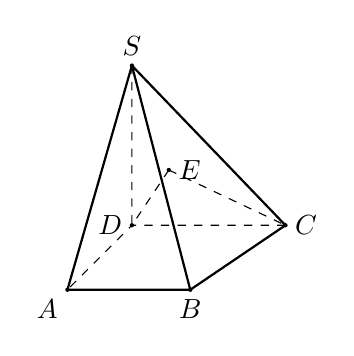
\begin{tikzpicture}[scale=.78,>=stealth]
\coordinate (A) at (0,0); \coordinate (B) at (2.0,0);
\coordinate (C) at (3.55,1.05); \coordinate (D) at (1.05,1.05);
\coordinate (S) at (1.05,3.65); \coordinate (E) at (1.65,1.95);
\draw[thick] (A)--(B)--(C);
\draw[dashed] (C)--(D)--(A) (S)--(D);
\draw[thick] (S)--(A) (S)--(B) (S)--(C);
\draw[dashed] (E)--(D) (E)--(C);
\fill (A) circle (1pt) node[below left] {$A$};
\fill (B) circle (1pt) node[below] {$B$};
\fill (C) circle (1pt) node[right] {$C$};
\fill (D) circle (1pt) node[left] {$D$};
\fill (S) circle (1pt) node[above] {$S$};
\fill (E) circle (1pt) node[right] {$E$};
\end{tikzpicture}
\end{center}
\nopagebreak[4]
（1） 证明：$SE=2EB$；

（2） 求二面角 $A-DE-C$ 的大小。

\Needspace{4\baselineskip}
\textbf{解析}

\gksubpart{(1)}

取 $D=(0,0,0)$、$C=(2,0,0)$、$A=(0,1,0)$、$B=(1,1,0)$、$S=(0,0,2)$，
设 $E=S+t(B-S)$。平面 $SBC$ 的法向量可取 $(1,1,1)$，平面 $EDC$ 的法向量
可取 $(0,-2(1-t),t)$。垂直条件给出 $3t-2=0$，即 $SE=2EB$。

\gksubpart{(2)}

此时平面 $ADE\text{、}CDE$ 的法向量可取 $(1,0,-1)$、$(0,-1,1)$，
按题目指定的两侧射线取二面角，余弦为 $-1/2$，故大小为 $120^\circ$。

\gkanswer{答案（1）：$SE=2EB$}

\gkanswer{答案（2）：二面角 $A-DE-C=120^\circ$。}

\end{answer}
\begin{answer}
\gksolhead{20}{}

\textbf{题目}：

已知函数 $f(x)=(x+1)\ln x-x+1$。

（1） 若 $xf'(x)\leq x^2+ax+1$，求 $a$ 的取值范围；

（2） 证明：$(x-1)f(x)\geq0$。

\Needspace{4\baselineskip}
\textbf{解析}

\gksubpart{(1)}

\Needspace{5\baselineskip}
由 $f'(x)=\ln x+1/x$，原不等式化为
\nopagebreak[4]
\[
\ln x\leq x+a.
\]
因为 $\ln x-x$ 的最大值为 $-1$，故 $a\geq-1$。

\gksubpart{(2)}

令 $h(x)=x\ln x+1$。其最小值为 $1-e^{-1}>0$，所以
$f'(x)=h(x)/x>0$，且 $f(1)=0$。因此 $f(x)$ 与 $x-1$ 同号，
$(x-1)f(x)\geq0$。

\gkanswer{答案（1）：$a\geq-1$。}

\gkanswer{答案（2）：见解析版}

\end{answer}
\begin{answer}
\gksolhead{21}{}

\textbf{题目}：

已知抛物线 $C:y^2=4x$ 的焦点为 $F$，过点 $K(-1,0)$ 的直线 $l$ 与 $C$ 相交于 $A\text{、}B$ 两点，点 $A$ 关于 $x$ 轴的对称点为 $D$。

（1） 证明：点 $F$ 在直线 $BD$ 上；

（2） 设 $\overrightarrow{FA}\cdot\overrightarrow{FB}=\dfrac89$，求 $\triangle BDK$ 的内切圆 $M$ 的方程。

\Needspace{4\baselineskip}
\textbf{解析}

\gksubpart{(1)}

设抛物线上参数点为 $(t^2,2t)$。过 $K(-1,0)$ 的弦两端参数为 $t$、$1/t$，
故 $A=(t^2,2t)$、$B=(t^{-2},2/t)$、$D=(t^2,-2t)$，焦点为 $F=(1,0)$。
\Needspace{5\baselineskip}
代入向量关系即可得到
\nopagebreak[4]
\[
\overrightarrow{FA}\cdot\overrightarrow{FB}=4-(t-t^{-1})^2=\frac89.
\]
这也直接说明 $F$ 在 $BD$ 上。

\gksubpart{(2)}

由上式 $(t+t^{-1})^2=64/9$。计算三角形 $BDK$ 的三边后，按边长加权
\Needspace{5\baselineskip}
求内心，得到内心为 $(1/9,0)$、内切半径为 $2/3$。故内切圆为
\nopagebreak[4]
\[
\left(x-\frac19\right)^2+y^2=\frac49.
\]

\gkanswer{答案（1）：见解析版}

\gkanswer{答案（2）：内切圆 $M$ 的方程为 $\left(x-\dfrac19\right)^2+y^2=\dfrac49$。}

\end{answer}
\begin{answer}
\gksolhead{22}{}

\textbf{题目}：

已知数列 $\{a_n\}$ 的前 $n$ 项和 $S_n=(n^2+n)\cdot3^n$。

（1） 求 $\displaystyle\lim_{n\to\infty}\dfrac{a_n}{S_n}$；

（2） 证明：$\displaystyle\frac{a_1}{1^2}+\frac{a_2}{2^2}+\cdots+\frac{a_n}{n^2}>3^n$。

\Needspace{4\baselineskip}
\textbf{解析}

\gksubpart{(1)}

\Needspace{5\baselineskip}
由 $S_n=(n^2+n)3^n$，作差得
\nopagebreak[4]
\[
a_n=S_n-S_{n-1}=2n(n+2)3^{n-1}\text{，}
\]
\Needspace{5\baselineskip}
从而
\nopagebreak[4]
\[
\frac{a_n}{S_n}=\frac{2(n+2)}{3(n+1)}\longrightarrow\frac23.
\]

\gksubpart{(2)}

\Needspace{5\baselineskip}
由上式
\nopagebreak[4]
\[
\frac{a_k}{k^2}=2\left(1+\frac2k\right)3^{k-1}>2\cdot3^{k-1}.
\]
求和得左端大于 $3^n-1$，而 $k=1$ 项额外贡献 $4$，故总和严格大于
$3^n$。

\gkanswer{答案（1）：$\displaystyle\lim_{n\to\infty}\dfrac{a_n}{S_n}=\dfrac23$。}

\gkanswer{答案（2）：见解析版}

\end{answer}